\section{Ka/Ks Analysis}

\subsection{Introduction}

\subsection{Methods}

\subsubsection{Calculation of dN/dS}

Selective constraints on gene sequence evolution were estimated using the dN/dS statistic calculated for orthologous group multiple sequence alignments. Protein sequence multiple alignments were generated first using Clustal-$\Omega$ \textcolor{red}{TODO CITE} and then used to inform CDS alignments with the codon-aware PAL2NAL alignment program \textcolor{red}{TODO CITE}.
%Ambiguous regions were removed from the CDS alignments using TrimAl (73), with the gap tolerance parameter set to 0.8 to exclude alignment columns with missing data in 20\% or more of the sequences in the orthologous group. Sequences were removed from the CDS alignments if more than 40% of their length was gap characters following multiple alignment.
Phylogenetic trees were constructed for each orthologous group using RAxML \textcolor{red}{TODO CITE} with a GTR+Gamma model of evolution. PAML v4.8 \textcolor{red}{TODO CITE} was used to calculate dN/dS ratios for each aligned orthologous group using the corresponding phylogenetic trees (codeml model=0, NSsites=0, ncatG=1). 

\begin{figure}[H]
  \centering
  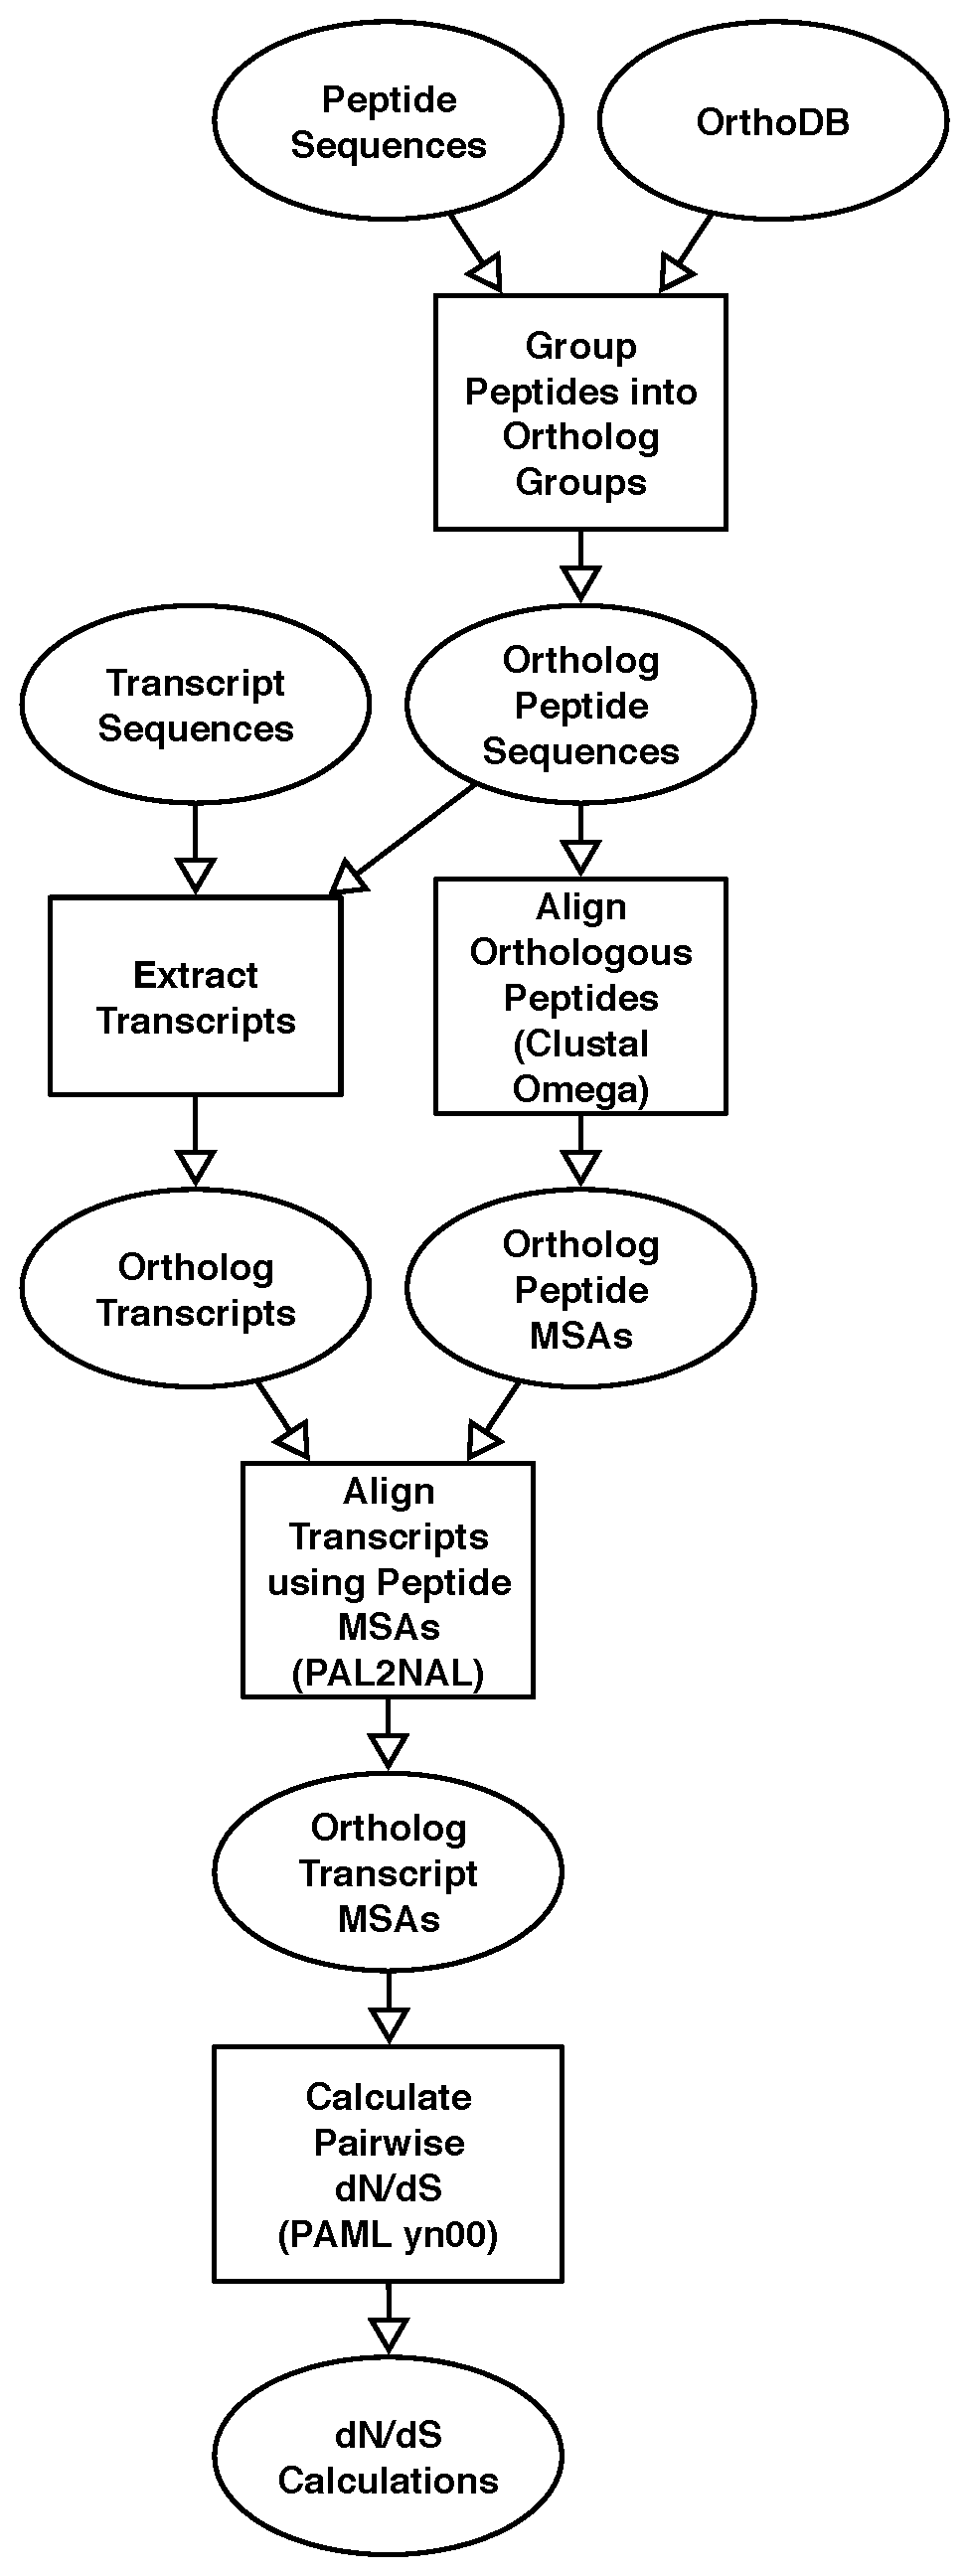
\includegraphics[width=0.25\textwidth]{figures/ka_ks/PAML_workflow}
  \caption{Workflow for Calculating dN/dS}
  \label{fig:ka-ks-workflow}
\end{figure}

\subsection{Results}

\subsubsection{Comparison of Opsins}

\subsubsection{Comparison of \emph{Drosophila} species}

\subsubsection{Comparison of \emph{L. longipalpis} and \emph{P. papatasi}}

\subsection{Discussion and Conclusion}